\subsection{Steering}
To steer the vehicle with a certain angle rate a servomotor is utilized. When the servomotor rotates to a specific angle, which is not the servo's middle position, it will pull on one of the brakes. Thus affecting the output of the differential gear and change the velocity on the belts placed on each side of the vehicle. The difference in belt velocities yields the angle of the moving vehicle.

\subsubsection{Brakes}
The moving vehicle turns by only pulling on one of it's brakes. if one of the belts is slower than the other it will make the vehicle turn regardless of changes in the motor output torque. A mechanical drawing of one of the brakes can be seen in \figref{Brakes}. 

 \begin{figure}[H]
	\centering
	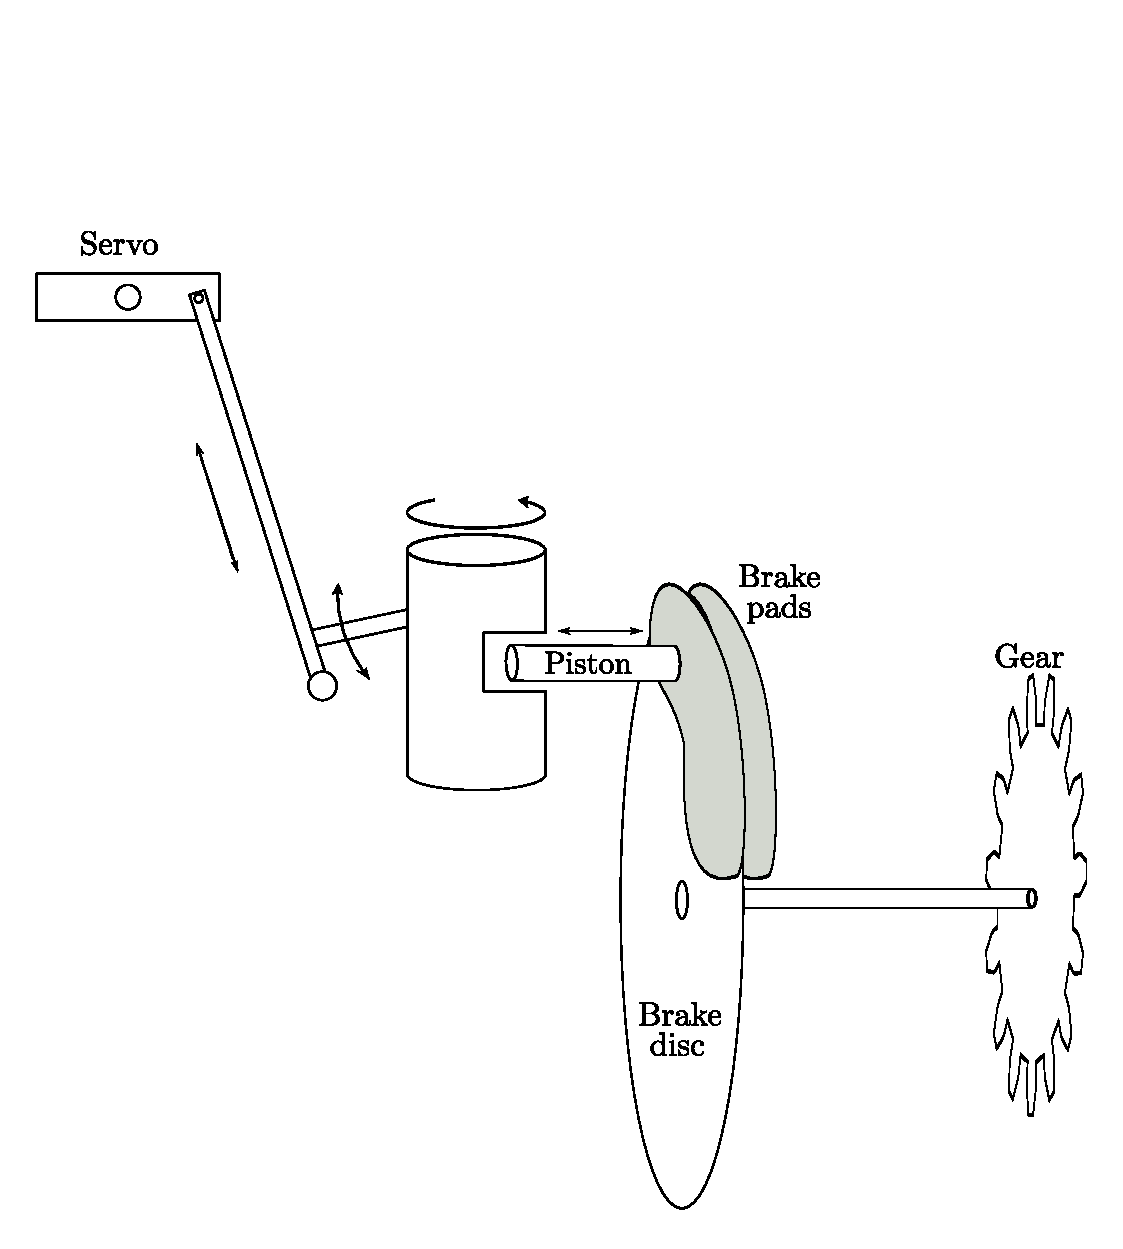
\includegraphics[scale=0.6]{figures/brakeDescription.pdf}
	\caption{Illustration of the brakes}
	\label{Brakes}
\end{figure}

When the servo rotate to a specific angle, it pulls an arm connected to a rotating cylinder, pushing the piston, seen in \figref{Brakes}, when it rotates. The piston pushes the brake pad closest to it and thereby adding friction to the brake disc.
